\documentclass[11pt]{article}
\usepackage[margin=1in]{geometry}
\usepackage[T1]{fontenc}
\usepackage{xcolor}
\usepackage{booktabs}
\usepackage{caption}
\usepackage{graphicx}
\usepackage{enumitem}
\usepackage{needspace}
\setlist[itemize]{itemsep=3pt, topsep=4pt}
\captionsetup{font=footnotesize, labelfont=bf}
\newcommand{\todo}[1]{\textcolor{red}{[TODO: #1]}}
\pagestyle{plain}

\title{Interpretable Biodegradability Screening\\[2pt] \large How Much Does Interpretability Cost?}
\author{\todo{Team names}}
\date{\todo{Date}}

\begin{document}
\maketitle

\section*{The problem}

Chemicals that do not break down in the environment can persist and accumulate, so many chemicals
must be assessed for \emph{ready biodegradability} before they are approved for use. The standard
laboratory tests are slow and costly, and the number of chemicals awaiting assessment is large.
Computational models that predict biodegradability from a chemical's structure can screen chemicals
before any lab work, so that tests are spent where they matter most.

\section*{Why the model must be interpretable}

A screening model is only useful if the people relying on it can trust and check it.
\begin{itemize}
  \item \textbf{Regulators need to justify decisions.} Guidance on using such models in chemical
        assessment asks for a clear algorithm and, where possible, a mechanistic interpretation
        \todo{cite the OECD principles for the validation of (Q)SAR models}. A prediction that says
        only ``not biodegradable'' is hard to defend; a rule such as ``more nitrogen and more
        branching, so likely persistent'' can be checked against chemistry.
  \item \textbf{Chemists need to act on the result.} A readable rule tells a chemist which
        structural features push a molecule toward persistence, which helps when designing greener
        alternatives.
  \item \textbf{Errors must be understandable.} When a readable model is wrong, one can see which
        condition led it astray and for which kinds of molecules it is unreliable.
\end{itemize}
Interpretability usually costs some accuracy. The open practical question is \emph{how much}, and
\emph{when the cost is small enough to accept}.

\section*{What this project does}

We use the UCI QSAR Biodegradation dataset (1,055 chemicals, 41 molecular descriptors, each
chemical labeled readily biodegradable, RB, or not, NRB) and compare nine models in two groups:
\begin{itemize}
  \item \textbf{Readable models:} CART and optimal classification trees (OCT), OCT-H (an optimal
        tree whose splits may combine several descriptors in a weighted sum), ridge logistic
        regression, and a sparse additive kernel model (a sum of one smooth curve per descriptor,
        which chooses at most $k$ descriptors itself by mixed-integer optimization).
  \item \textbf{Flexible models} that make no attempt to be readable: random forest, XGBoost,
        Gaussian-kernel logistic regression and Nadaraya--Watson kernel regression. They show how
        well \emph{any} model can do with the same descriptors, so the gap to them is the price of
        readability.
\end{itemize}
Models are compared at four descriptor budgets (3, 5, 10 and all 41) and at two decision
thresholds: one balancing both types of error, and a cautious one that catches at least 90\% of
non-biodegradable chemicals.

\section*{How the models were compared}

\begin{itemize}
  \item \textbf{Data split.} A stratified 60/20/20 split (identical descriptor rows kept together).
        Training and validation are combined into one development set of 844 chemicals (559 NRB,
        285 RB); the 211 test chemicals are set aside and have not been used.
  \item \textbf{Cross-validation.} Every model uses the same stratified 5-fold split of the
        development set. Each setting is fit on four folds and scored on the fifth; settings are
        chosen by mean cross-validated AUC, and the chosen setting is refit on all 844 chemicals.
        For trees (depth 2--4, minimum leaf size 5, 10 or 20), the simplest setting within 0.01 AUC
        of the best is taken.
  \item \textbf{Descriptor budgets.} The 3-, 5- and 10-descriptor lists come from exact best-subset
        selection (least squares on standardized descriptors) on the development set, and every
        model uses the same lists. The one exception is the additive kernel model, which picks its
        own $k$ descriptors inside every fold, so the held-out chemicals never influence its choice.
  \item \textbf{Thresholds.} Both decision thresholds are set on out-of-fold predictions, where
        each chemical is scored by a model that never saw it. Plain accuracy is not reported because
        always predicting NRB already scores 66\%.
\end{itemize}

\section*{What the descriptors carry}

\begin{itemize}
  \item \textbf{The 41 descriptors carry about six underlying properties.} Seventeen pairs have
        Spearman correlation above 0.8, forming six groups. The two largest are
        \emph{size and branching} (SpMax\_L, SpMax\_A, SM6\_L, SpMax\_B(m), SM6\_B(m), HyWi\_B(m))
        and \emph{nitrogen content} (nN, F02[C-N], F03[C-N], F04[C-N]); smaller groups cover
        composition, oxygen, electronegativity and bromine.
  \item \textbf{No descriptor is strong on its own.} The strongest, SpMax\_B(m), has correlation
        0.50 with NRB, and the top six all come from the size or composition groups: larger,
        heavier, more branched molecules tend to be persistent. Good prediction needs several
        properties combined.
  \item \textbf{Ten descriptors are rare flags}, zero for more than 85\% of chemicals (for example
        nArNO2, nCRX3): decisive for the few chemicals that have them, minor on average.
  \item \textbf{Sparse selection keeps about one descriptor per property.} The 3-descriptor list is
        SpMax\_L, LOC and SpPosA\_B(p); the 5-descriptor list adds nitrogen and oxygen counts.
        Which member of a group is picked is close to arbitrary, so a split on SpMax\_L should be
        read as ``larger, more branched molecule'', not as one exact descriptor.
\end{itemize}

\needspace{12\baselineskip}
\section*{What the results show}

\begin{table}[t]
\centering
\small
\begin{tabular}{l cccc c cccc}
\toprule
 & \multicolumn{4}{c}{Cross-validated AUC} & & \multicolumn{4}{c}{RB chemicals cleared (of 285)} \\
\cmidrule{2-5} \cmidrule{7-10}
Model & $k=3$ & $k=5$ & $k=10$ & all 41 & & $k=3$ & $k=5$ & $k=10$ & all 41 \\
\midrule
\multicolumn{10}{l}{\emph{Flexible models}} \\
Random forest        & 0.855 & \textbf{0.917} & \textbf{0.932} & 0.942 & & 157 & 216 & 216 & 233 \\
XGBoost              & 0.851 & 0.915 & 0.924 & 0.941 & & 148 & \textbf{217} & 218 & 232 \\
Kernel logistic      & 0.849 & 0.910 & 0.929 & \textbf{0.943} & & 156 & 209 & 221 & \textbf{239} \\
Nadaraya--Watson     & 0.840 & 0.891 & 0.910 & 0.915 & & 155 & 202 & 212 & 224 \\
\midrule
\multicolumn{10}{l}{\emph{Readable models}} \\
Additive kernel$^\dagger$ & \textbf{0.878} & 0.904 & 0.919 & 0.936 & & \textbf{184} & 208 & 217 & 226 \\
Ridge logistic       & 0.830 & 0.881 & 0.910 & 0.931 & & 157 & 179 & \textbf{223} & 226 \\
OCT-H                & 0.806 & 0.866 & 0.866 & 0.875 & & 125 & 210 & 210 & 219 \\
OCT                  & 0.792 & 0.842 & 0.830 & 0.834 & & 126 & 167 & 190 & 149 \\
CART                 & 0.819 & 0.809 & 0.823 & 0.828 & & 105 & 175 & 177 & 186 \\
\bottomrule
\end{tabular}
\caption{Out-of-fold results on 844 development chemicals; best per column in bold. ``RB
cleared'': readily biodegradable chemicals correctly spared a lab test when each model is set to
catch at least 90\% of non-biodegradable ones (higher means fewer unnecessary tests). Fold-to-fold
spread in AUC is about $\pm 0.01$--$0.04$. $^\dagger$Chooses its own $k$ descriptors within each
fold instead of using the fixed lists.}
\end{table}

\begin{figure}[t]
\centering
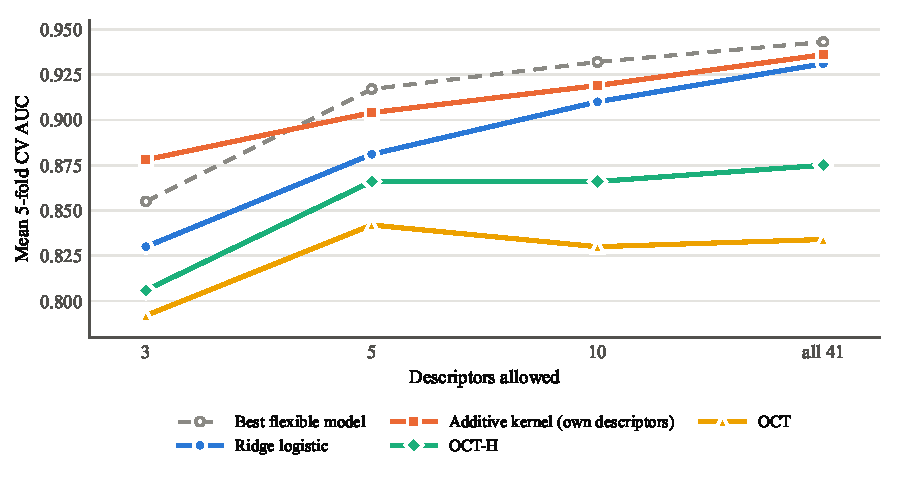
\includegraphics[width=0.92\textwidth]{figures/auc_by_budget.pdf}
\caption{Mean cross-validated AUC by descriptor budget. The dashed line is the best flexible model
(random forest, XGBoost or kernel logistic) at each budget; the gap below it is the price of
readability. CART, omitted for clarity, stays between 0.81 and 0.83 (Table~1).}
\end{figure}

\paragraph{The cost of interpretability grows with the descriptor budget.}
\begin{itemize}
  \item \textbf{The flexible models agree on a ceiling.} Random forest, XGBoost and kernel logistic
        regression land within about one fold-to-fold spread of each other at every budget (AUC
        about 0.85, 0.92, 0.93 and 0.94), so this is a fair estimate of how much the descriptors
        can predict. Nadaraya--Watson, a pure local average, falls 0.01--0.03 below it, most with all
        41 descriptors, where ``nearest'' chemicals in 41 dimensions are not very near.
  \item \textbf{Logistic regression is close to the ceiling when many descriptors are allowed.} It
        trails by 0.012 AUC with all 41 and 0.022 at $k=10$, but by 0.036 at $k=5$.
  \item \textbf{Axis-aligned trees fall further behind as descriptors are added.} OCT and CART stay
        between 0.79 and 0.84 AUC at every budget, so their gap to the ceiling widens from
        0.04--0.06 at $k=3$ to about 0.11 with all 41. The signal is spread across several
        properties, each only moderately linked to persistence; a weighted sum gains a little from
        every extra descriptor, but a depth-4 tree can use only a handful (the OCT on all 41 uses 8).
  \item \textbf{Depth is not what holds trees back.} Depth 2 is always too shallow (AUC 0.73--0.77);
        going from depth 3 to 4 still adds 0.02--0.03 AUC, but leaves grow from about 6 to 8--11.
        Even at that rate, closing the 0.09 gap to logistic regression with all 41 would take
        several more levels and a tree too large to explain.
\end{itemize}

\paragraph{Which readable model to trust depends on the budget.}
\begin{itemize}
  \item \textbf{At three descriptors, which descriptors are used matters most.} The additive kernel
        model picks SpMax\_L, SpPosA\_B(p) and nN (the fixed list has LOC instead of nN) and is the
        best model at $k=3$: AUC 0.878 and 184 chemicals cleared, 27 more than any model on the
        fixed list. On the fixed list, logistic regression matches the best flexible model at the
        cautious threshold (157 cleared), and the trees clear only 105--126.
  \item \textbf{At five descriptors, OCT-H nearly matches the flexible models for screening.} Set to
        catch 90\% of persistent chemicals, it clears 210 of 285 biodegradable chemicals, against
        202--217 for the flexible models, 179 for logistic regression and 167--175 for OCT and CART.
        The tree has 7 leaves, and each split is a weighted sum of the same five descriptors.
  \item \textbf{With ten or more descriptors, logistic regression is the readable choice.} It is
        within 0.01--0.02 AUC of the ceiling and clears 223--226 chemicals; OCT-H gains 0.03--0.04
        AUC over the OCT but its all-41 tree, though only 4 leaves, uses 26 descriptors in its splits
        and cannot be checked by hand.
  \item \textbf{OCT and CART perform similarly.} The OCT is clearly ahead only at $k=5$ (AUC 0.842
        against 0.809) and CART at $k=3$; elsewhere they are within one fold-to-fold spread. The OCT
        is not smaller, but it is more stable across folds (spread about 0.02, against up to 0.04).
\end{itemize}

\paragraph{The cautious threshold widens the gap for trees.} A tree's threshold moves in
leaf-sized steps, so reaching 90\% recall often means flagging a whole mixed leaf with many
biodegradable chemicals. The OCT with all 41 descriptors clears 77 fewer biodegradable chemicals
than logistic regression at that threshold, a larger gap than its balanced accuracy suggests
(Table~2). At $k=3$ the OCT has competitive balanced accuracy (0.774 against 0.763 for logistic
regression) but clears only 126 chemicals once it must catch 90\% of persistent ones, against 157.

\begin{table}[t]
\centering
\small
\begin{tabular}{l cccc c cccc}
\toprule
 & \multicolumn{4}{c}{Balanced accuracy} & & \multicolumn{4}{c}{Tree leaves} \\
\cmidrule{2-5} \cmidrule{7-10}
Model & $k=3$ & $k=5$ & $k=10$ & all 41 & & $k=3$ & $k=5$ & $k=10$ & all 41 \\
\midrule
Random forest        & 0.791 & \textbf{0.839} & \textbf{0.851} & 0.871 & & & & & \\
XGBoost              & 0.787 & 0.837 & 0.839 & 0.865 & & & & & \\
Kernel logistic      & 0.788 & 0.836 & 0.848 & \textbf{0.875} & & & & & \\
Nadaraya--Watson     & 0.778 & 0.817 & 0.840 & 0.861 & & & & & \\
\midrule
Additive kernel$^\dagger$ & \textbf{0.799} & 0.831 & 0.849 & 0.863 & & & & & \\
Ridge logistic       & 0.763 & 0.806 & 0.844 & 0.868 & & & & & \\
OCT-H                & 0.769 & 0.822 & 0.821 & 0.842 & & 6 & 7 & 5 & 4 \\
OCT                  & 0.774 & 0.813 & 0.788 & 0.789 & & 6 & 9 & 8 & 9 \\
CART                 & 0.787 & 0.771 & 0.785 & 0.812 & & 6 & 5 & 6 & 7 \\
\bottomrule
\end{tabular}
\caption{Out-of-fold balanced accuracy (mean of NRB recall and RB specificity) at each model's
balanced threshold, and the number of leaves in each final tree. $^\dagger$Chooses its own $k$
descriptors within each fold.}
\end{table}

\section*{What the results let people do}

\begin{itemize}
  \item \textbf{Judge interpretability against the right baseline.} The gap to the flexible-model
        ceiling is the real price of readability; Table~1 gives it for each budget, in AUC and in
        extra lab tests.
  \item \textbf{Pick the readable model that fits the budget.}
        \begin{itemize}[itemsep=1pt]
          \item \emph{3 descriptors:} the additive kernel model, which can be read as three curves,
                one per descriptor; among models on the fixed list, logistic regression.
          \item \emph{5 descriptors:} OCT-H, if a tree-shaped rule is wanted and a short calculation
                at each split is acceptable; it costs at most 7 extra tests against the best flexible
                model. Requiring single-descriptor splits (OCT or CART) costs about 40--50 more.
          \item \emph{10 or more descriptors:} logistic regression, within 0.01--0.02 AUC of the
                ceiling and still transparent; trees fall well behind.
        \end{itemize}
  \item \textbf{Know what dropping interpretability buys.} With all 41 descriptors, kernel logistic
        regression clears 239 biodegradable chemicals at the cautious threshold against 226 for
        logistic regression: 13 fewer unnecessary tests out of 285.
  \item \textbf{Read the models at the level of chemical properties.} Because the descriptors carry
        about six properties, a split such as ``SpMax\_L $\geq$ 5.1'' should be read as ``larger,
        more branched molecule'', and logistic weights within a group cannot be read one by one.
  \item \textbf{Judge methods fairly.} Comparing optimal and greedy trees under cross-validation
        shows that a single validation split can overstate a method's advantage; the two perform
        similarly, with optimal trees more stable.
\end{itemize}

\section*{Expected impact}

\begin{itemize}
  \item \textbf{For screening labs and regulators:} a quantified answer to whether an interpretable
        screen is acceptable for a given number of descriptors, and how many extra tests it costs.
  \item \textbf{For chemists:} readable rules linking molecular properties to persistence, useful
        as a first check and as design guidance.
  \item \textbf{For practitioners of interpretable machine learning:} a worked example showing that
        the cost of interpretability depends on how much information a model is allowed to use,
        measured against a ceiling set by flexible models, with careful validation.
\end{itemize}

\section*{Limits of the contribution}

\begin{itemize}
  \item \textbf{Cross-validation only.} All results are out-of-fold on the development set; the
        test set is held back until every setting is frozen.
  \item \textbf{Associations, not causes.} The rules describe associations within one public
        dataset of 1,055 chemicals.
  \item \textbf{Screening aids, not replacements.} At balanced accuracy of about 0.76--0.88, the
        models prioritize chemicals for testing; they do not replace laboratory tests. The
        contribution is the trade-off analysis, not a new state-of-the-art accuracy on this
        well-studied dataset.
  \item \textbf{Small differences are not reliable.} AUC gaps below about 0.02 are within
        fold-to-fold spread, and the cleared counts have no error bars.
  \item \textbf{Slightly optimistic estimates.} The fixed descriptor lists were chosen on all 844
        development chemicals, flattering every model that uses them equally; the flexible models
        were tuned over small grids, so the true ceiling may be slightly higher.
  \item \textbf{The additive model's descriptor choice is not proven optimal.} The optimization's
        lower bound converges slowly, so each search stops after 50 cutting planes and finishes with
        a local search; only the final $k=3$ choice is proven optimal, and the other searches have
        a median remaining gap of 20\%. Its choices vary between folds at $k=3$ and 10 (they are
        stable at $k=5$), and its advantage at $k=3$ may come from its descriptors rather than its
        form, since it does not use the fixed lists.
\end{itemize}

\end{document}
